\documentclass[preprint,12pt,aps,pra,showkeys,amsmath,amssymb,superscriptaddress,floatfix]{revtex4-2}
\usepackage[T1]{fontenc}
\usepackage[utf8]{inputenc}
\usepackage{amsmath,amssymb,amsthm,mathtools,mathrsfs}
\usepackage{microtype,booktabs,enumitem}
\usepackage{xcolor,tikz,etoolbox}
\usepackage[skins,breakable]{tcolorbox}
\usepackage{needspace}
% Keep diagram geometry independent of REVTeX preprint body spacing.
\AtBeginEnvironment{tikzpicture}{\linespread{1}\selectfont}
\usetikzlibrary{arrows.meta,positioning,calc,fit,decorations.pathreplacing}
\usepackage{graphicx}
\usepackage{hyperref}

\definecolor{MMBlue}{RGB}{0,82,155}
\definecolor{MMOrange}{RGB}{200,80,0}
\tikzset{
 mmnode/.style={draw=MMBlue,rounded corners=2pt,fill=MMBlue!4,align=left,execute at begin node={\raggedright},text width=5cm,font=\fontsize{10}{12}\selectfont,inner sep=6pt},
 mmimport/.style={mmnode,draw=black!65,fill=black!4},
 mmcandidate/.style={mmnode,draw=MMOrange,dashed,fill=MMOrange!5},
 mmrejected/.style={mmnode,draw=black,densely dotted,fill=black!8},
 mmproof/.style={->,thick,MMBlue},
 mmflow/.style={->,semithick,black!70},
 mmrepair/.style={->,dashed,thick,MMOrange},
 mmcandidatearrow/.style={->,dashed,semithick,MMOrange},
 mmnote/.style={font=\scriptsize,fill=white,inner sep=2pt,align=center}}

\usepackage[section]{placeins}
\setlength{\emergencystretch}{3em}
\setlist{itemsep=3pt,topsep=4pt}
\newtheorem{theorem}{Theorem}[section]
\newtheorem{proposition}[theorem]{Proposition}
\newtheorem{lemma}[theorem]{Lemma}
\newtheorem{corollary}[theorem]{Corollary}
\theoremstyle{definition}
\newtheorem{definition}[theorem]{Definition}
\newtheorem{example}[theorem]{Example}
\theoremstyle{remark}
\newtheorem{remark}[theorem]{Remark}
% Avoid isolated statement headings and single-line paragraph fragments.
\BeforeBeginEnvironment{theorem}{\Needspace{6\baselineskip}}
\BeforeBeginEnvironment{definition}{\Needspace{5\baselineskip}}
\BeforeBeginEnvironment{proposition}{\Needspace{5\baselineskip}}
\BeforeBeginEnvironment{lemma}{\Needspace{5\baselineskip}}
\BeforeBeginEnvironment{corollary}{\Needspace{5\baselineskip}}
\clubpenalty=5000
\widowpenalty=5000
\newcommand{\R}{\mathbb R}\newcommand{\Z}{\mathbb Z}\newcommand{\N}{\mathbb N}
\newcommand{\Pa}{\operatorname{Pa}}\newcommand{\Desc}{\operatorname{Desc}}
\newcommand{\cl}{\operatorname{cl}}\newcommand{\cost}{\operatorname{cost}}
\newcommand{\status}{\operatorname{status}}
% Faculty cards: a visual rail groups the five faculties within one agent.
% The rail has no arrowhead and does not represent a proof dependency.
\newcommand{\mmfacultybadge}[1]{%
 \node[circle,draw=MMBlue,line width=1pt,fill=white,
 minimum size=7mm,inner sep=0pt,font=\sffamily\small\bfseries,text=MMBlue]
 at ([xshift=15pt,yshift=-15pt]frame.north west) {#1};}
\newcommand{\mmfacultyrail}{%
 \draw[MMBlue!80,line width=1pt]
 ([xshift=15pt,yshift=2pt]frame.north west)--
 ([xshift=15pt,yshift=-2pt]frame.south west);}
\newtcolorbox{mmfacultybox}[2]{enhanced,breakable,
 colback=MMBlue!4,colframe=MMBlue!4,boxrule=0pt,arc=3pt,
 left=39pt,right=9pt,top=4pt,bottom=4pt,
 before skip=2pt,after skip=2pt,
 fontupper=\small\linespread{1.1}\selectfont,
 overlay unbroken={\mmfacultyrail\mmfacultybadge{#1}},
 overlay first={\mmfacultyrail\mmfacultybadge{#1}},
 overlay middle={\mmfacultyrail},overlay last={\mmfacultyrail}}
\newcommand{\mmfaculty}[3]{%
 \begin{mmfacultybox}{#1}{#2}
 {\sffamily\bfseries\color{MMBlue}#2}\par\smallskip #3
 \end{mmfacultybox}}
\newcommand{\agent}[9]{%
 \Needspace{8\baselineskip}
 \subsubsection{#1}
 \noindent\textbf{Object.} #2\par
 \noindent\textbf{Role.} #3\par\smallskip
 \mmfaculty{E}{Ego}{#4}
 \mmfaculty{M}{Memory}{#5}
 \mmfaculty{I}{Intellect}{#6}
 \mmfaculty{S}{Sense}{#7}
 \mmfaculty{A}{Action}{#8}
 \smallskip\noindent #9\par}

\usepackage{longtable,array,calc}
\providecommand{\tightlist}{\setlength{\itemsep}{2pt}\setlength{\parskip}{0pt}}
\makeatletter
\def\frontmatter@abstract@produce{\par\addvspace{\frontmatter@preabstractspace}%
\begingroup\prep@absbox\unvbox\absbox\post@absbox\endgroup
\addvspace{\frontmatter@postabstractspace}}
\makeatother
\newcommand{\field}[2]{\par\smallskip\noindent\textbf{#1.} #2\par}
\setlength{\emergencystretch}{5em}
\AtBeginEnvironment{verbatim}{\small\linespread{1.0}\selectfont}


\hypersetup{colorlinks=true,linkcolor=MMBlue,urlcolor=MMBlue,pdfauthor={Dibakar Sigdel}}

\begin{document}

\title{Finite-Dimensional Irreducible Representations of sl2\\[4pt]\large An End-to-End Meta-Math Walkthrough}

\author{Dibakar Sigdel}

\affiliation{Mindverse Computing LLC, Lynnwood, WA 98087, USA}

\date{October 2026}

\begin{abstract}

Raising must eventually stop because it creates distinct weights.
Lowering from a highest-weight vector then forces the highest weight to
be a nonnegative integer. The report presents the target theorem,
declared imports, a dependency graph, five-faculty node contracts, a
continuous proof, a worked example, and a hypothesis-repair audit. It is
an authored mathematical exposition, not a deployed-agent transcript or
a formal proof-assistant certificate.

\end{abstract}\maketitle\linespread{1.12}\selectfont

\noindent\textbf{RT-05 / Representation Theory and Lie Theory / Report v1}

\section{Target and import contract}

\begin{theorem}

Let \(\mathfrak{sl}_2(\mathbb C)\) have generators \(e,f,h\) satisfying
\([h,e]=2e\), \([h,f]=-2f\), and \([e,f]=h\). Every nonzero
finite-dimensional irreducible representation is, up to isomorphism,
exactly one \(V_n\) for an integer \(n\ge0\). It has basis
\(v_0,\ldots,v_n\) with \(hv_j=(n-2j)v_j\), \(fv_j=v_{j+1}\) (and
\(fv_n=0\)), and \(ev_j=j(n-j+1)v_{j-1}\) (and \(ev_0=0\)). In
particular \(\dim V_n=n+1\).

\end{theorem}

\subsection{Foundations and permitted imports}

Use eigenvalue existence over \(\mathbb C\), linear independence of
eigenvectors for distinct eigenvalues, the displayed Lie brackets, and
polynomial interpolation on finitely many distinct scalars.
Irreducibility is assumed for classification; this project does not
prove that every finite-dimensional representation is completely
reducible.

\clearpage\section{Node interaction workflow}

\begin{center}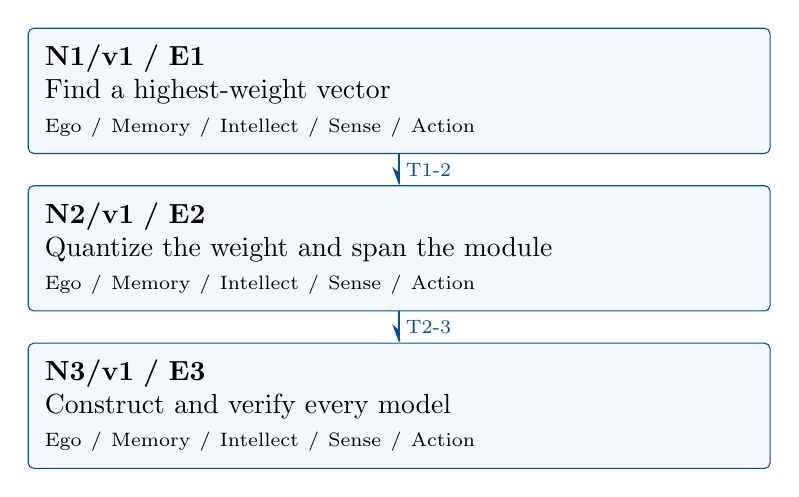
\begin{tikzpicture}[>=Stealth,x=1cm,y=1cm]

\node[mmnode,text width=9cm,minimum height=1.25cm] (N1) at (0,0.0) {\textbf{N1/v1 / E1}\\Find a highest-weight vector\\{\scriptsize Ego / Memory / Intellect / Sense / Action}};

\node[mmnode,text width=9cm,minimum height=1.25cm] (N2) at (0,-2.0) {\textbf{N2/v1 / E2}\\Quantize the weight and span the module\\{\scriptsize Ego / Memory / Intellect / Sense / Action}};

\node[mmnode,text width=9cm,minimum height=1.25cm] (N3) at (0,-4.0) {\textbf{N3/v1 / E3}\\Construct and verify every model\\{\scriptsize Ego / Memory / Intellect / Sense / Action}};

\draw[mmproof] (N1.south) -- node[mmnote,right] {T1-2} (N2.north);

\draw[mmproof] (N2.south) -- node[mmnote,right] {T2-3} (N3.north);

\end{tikzpicture}\end{center}

Each box is one mathematical agent containing all five faculties. Blue
arrows carry the versioned exports listed below. The layout gives a
reading order; only drawn arrows assert dependencies. Diagnostic repair
is separate from the proof DAG.

\subsection{Versioned evidence-transfer ledger}

\begingroup\small\linespread{1.05}\selectfont

\Needspace{5\baselineskip}\field{T1-2: N1/E1/v1 to N2}{There is \(v_0\ne0\) with \(ev_0=0\) and \(hv_0=\lambda v_0\) for some
\(\lambda\in\mathbb C\).}

\field{Receiving activity}{N2.1}

\field{Compatibility}{E1/v1 and irreducibility of \(V\); write \(v_j=f^jv_0\). Check: The
coefficient equation at \(v_{n+1}=0\) uses \(v_n\ne0\) and
characteristic zero.}

\Needspace{5\baselineskip}\field{T2-3: N2/E2/v1 to N3}{\(\lambda=n\in\mathbb Z_{\ge0}\) and \(v_0,\ldots,v_n\) form a basis of
\(V\) with the stated actions.}

\field{Receiving activity}{N3.3}

\field{Compatibility}{An arbitrary integer \(n\ge0\) and the formulas in the theorem. Check:
Existence and irreducibility of the proposed models must be established
in addition to the classification of a given module.}

\endgroup

\clearpage\section{Agent roles and five-faculty activities}\begingroup\small\linespread{1.05}\selectfont\setlist{itemsep=1pt,topsep=2pt}

\subsection{N1/v1: Find a highest-weight vector}

\field{Object and role}{Start with an \(h\)-eigenvector and raise it until the last nonzero
term. \textbf{Local obligation:} There is \(v_0\ne0\) with \(ev_0=0\)
and \(hv_0=\lambda v_0\) for some \(\lambda\in\mathbb C\).}

\field{Inputs}{A nonzero finite-dimensional representation \(V\).}

\mmfaculty{E}{Ego}{Publish E1/v1 only after establishing this obligation: There is
\(v_0\ne0\) with \(ev_0=0\) and \(hv_0=\lambda v_0\) for some
\(\lambda\in\mathbb C\).}

\mmfaculty{M}{Memory}{A nonzero finite-dimensional representation \(V\). Retain the stated
assumptions and import versions.}

\mmfaculty{I}{Intellect}{Start with an \(h\)-eigenvector and raise it until the last nonzero
term.}

\mmfaculty{S}{Sense}{The raising chain has distinct weights; finite-dimensionality, not a
preassumed diagonalization of all of \(h\), forces termination.}

\mmfaculty{A}{Action}{Carry out activities N1.1--N1.2 below, retaining each calculation and
construction as evidence.}

\smallskip\noindent\textbf{Numbered mathematical activities}

\begin{enumerate}[label=N1.\arabic*,leftmargin=3.4em]

\item Choose \(w\ne0\) with \(hw=\alpha w\). The relation \(he=eh+2e\) gives
\(h(e^jw)=(\alpha+2j)e^jw\) by induction. Nonzero members of this
sequence are eigenvectors with distinct eigenvalues and hence linearly
independent.

\item They cannot all be nonzero in finite dimension. Choose the last nonzero
one before the first zero, and name it \(v_0\). It is killed by \(e\)
and has an \(h\)-eigenvalue \(\lambda\), as required.

\end{enumerate}

\field{Export E1/v1}{There is \(v_0\ne0\) with \(ev_0=0\) and \(hv_0=\lambda v_0\) for some
\(\lambda\in\mathbb C\).}

\field{Acceptance gate}{The raising chain has distinct weights; finite-dimensionality, not a
preassumed diagonalization of all of \(h\), forces termination.}

\field{Targeted repair}{If \(h\) is declared diagonalizable at the outset, replace that unproved
claim by one eigenvector and the finite raising chain. Withhold this
export and recheck its descendants after a versioned correction.}

\clearpage

\subsection{N2/v1: Quantize the weight and span the module}

\field{Object and role}{Commute \(e\) through powers of \(f\) and inspect the first vanishing
lowered vector. \textbf{Local obligation:}
\(\lambda=n\in\mathbb Z_{\ge0}\) and \(v_0,\ldots,v_n\) form a basis of
\(V\) with the stated actions.}

\field{Inputs}{E1/v1 and irreducibility of \(V\); write \(v_j=f^jv_0\). Incoming proof
exports: E1/v1 at N2.1.}

\mmfaculty{E}{Ego}{Publish E2/v1 only after establishing this obligation:
\(\lambda=n\in\mathbb Z_{\ge0}\) and \(v_0,\ldots,v_n\) form a basis of
\(V\) with the stated actions.}

\mmfaculty{M}{Memory}{E1/v1 and irreducibility of \(V\); write \(v_j=f^jv_0\). Incoming proof
exports: E1/v1 at N2.1. Retain the stated assumptions and import
versions.}

\mmfaculty{I}{Intellect}{Commute \(e\) through powers of \(f\) and inspect the first vanishing
lowered vector.}

\mmfaculty{S}{Sense}{The coefficient equation at \(v_{n+1}=0\) uses \(v_n\ne0\) and
characteristic zero.}

\mmfaculty{A}{Action}{Carry out activities N2.1--N2.3 below, retaining each calculation and
construction as evidence.}

\smallskip\noindent\textbf{Numbered mathematical activities}

\begin{enumerate}[label=N2.\arabic*,leftmargin=3.4em]

\item Inductively, \(hv_j=(\lambda-2j)v_j\). Also \(ev_0=0\) and
\(ev_{j+1}=efv_j=fev_j+hv_j\), so induction gives
\(ev_j=j(\lambda-j+1)v_{j-1}\). These identities use only the brackets
and remain true until and including the first zero vector.

\item The nonzero lowered vectors have distinct weights, so finite dimension
gives a largest \(n\) with \(v_n\ne0\) and \(v_{n+1}=0\). Applying the
formula at \(n+1\) yields \(0=(n+1)(\lambda-n)v_n\). Therefore
\(\lambda=n\).

\item The span of \(v_0,\ldots,v_n\) is invariant under \(e,f,h\) by these
formulas and is nonzero. Irreducibility forces it to equal \(V\).
Distinct weights give linear independence, so these vectors are a basis
and all claimed coefficients follow.

\end{enumerate}

\field{Export E2/v1}{\(\lambda=n\in\mathbb Z_{\ge0}\) and \(v_0,\ldots,v_n\) form a basis of
\(V\) with the stated actions.}

\field{Acceptance gate}{The coefficient equation at \(v_{n+1}=0\) uses \(v_n\ne0\) and
characteristic zero.}

\field{Targeted repair}{If termination of lowering is asserted without justification, use the
distinct eigenvalues; then apply the formula at the first zero, not
merely at \(v_n\). Withhold this export and recheck its descendants
after a versioned correction.}

\clearpage

\begingroup\linespread{1}\fontsize{9.5}{11}\selectfont\renewcommand{\small}{\fontsize{9.5}{11}\selectfont}

\subsection{N3/v1: Construct and verify every model}

\field{Object and role}{Check the brackets directly and recover the highest vector from any
nonzero invariant subspace. \textbf{Local obligation:} For each \(n\),
\(V_n\) exists and is irreducible; these exhaust all isomorphism classes
without duplication.}

\field{Inputs}{An arbitrary integer \(n\ge0\) and the formulas in the theorem. Incoming
proof exports: E2/v1 at N3.3.}

\mmfaculty{E}{Ego}{Publish E3/v1 only after establishing this obligation: For each \(n\),
\(V_n\) exists and is irreducible; these exhaust all isomorphism classes
without duplication.}

\mmfaculty{M}{Memory}{An arbitrary integer \(n\ge0\) and the formulas in the theorem. Incoming
proof exports: E2/v1 at N3.3. Retain the stated assumptions and import
versions.}

\mmfaculty{I}{Intellect}{Check the brackets directly and recover the highest vector from any
nonzero invariant subspace.}

\mmfaculty{S}{Sense}{Existence and irreducibility of the proposed models must be established
in addition to the classification of a given module.}

\mmfaculty{A}{Action}{Carry out activities N3.1--N3.3 below, retaining each calculation and
construction as evidence.}

\smallskip\noindent\textbf{Numbered mathematical activities}

\begin{enumerate}[label=N3.\arabic*,leftmargin=3.4em]

\item Define three linear maps on the abstract basis by the stated formulas.
The weight differences give \([h,e]=2e\) and \([h,f]=-2f\). Direct
subtraction gives \([e,f]v_j=((j+1)(n-j)-j(n-j+1))v_j=(n-2j)v_j=hv_j\),
with the same result at \(j=0,n\) using zero boundary terms. Thus they
define a representation.

\item Let \(U\) be a nonzero invariant subspace. A nonzero vector of \(U\) has
a nonzero component along some \(v_j\). Because the \(h\)-eigenvalues
are distinct, a polynomial in \(h\) that equals one at that weight and
zero at the other weights extracts a nonzero multiple of \(v_j\) within
\(U\). Applying \(e^j\) gives a nonzero multiple of \(v_0\), since all
coefficients \(r(n-r+1)\) for \(1\le r\le j\) are nonzero. Repeated
\(f\) then yields every basis vector. Hence \(U=V_n\).

\item N2 identifies any irreducible module with its corresponding model by
sending the displayed basis to the abstract one. Different \(n\) give
different dimensions, so the models are pairwise nonisomorphic. This
proves existence, uniqueness, and exhaustion.

\end{enumerate}

\field{Export E3/v1}{For each \(n\), \(V_n\) exists and is irreducible; these exhaust all
isomorphism classes without duplication.}

\field{Acceptance gate}{Existence and irreducibility of the proposed models must be established
in addition to the classification of a given module.}

\field{Targeted repair}{If only the possible highest weights have been listed, add bracket
verification and the invariant-subspace argument to establish that every
listed model really exists and is irreducible. Withhold this export and
recheck its descendants after a versioned correction.}

\endgroup

\endgroup\clearpage\section{Continuous mathematical proof}\label{sec:proof}

\subsection{N1 --- Find a highest-weight
vector}\label{n1-find-a-highest-weight-vector}

\begin{enumerate}
\def\labelenumi{\arabic{enumi}.}
\item
  \textbf{N1.1.} Choose \(w\ne0\) with \(hw=\alpha w\). The relation
  \(he=eh+2e\) gives \(h(e^jw)=(\alpha+2j)e^jw\) by induction. Nonzero
  members of this sequence are eigenvectors with distinct eigenvalues
  and hence linearly independent.
\item
  \textbf{N1.2.} They cannot all be nonzero in finite dimension. Choose
  the last nonzero one before the first zero, and name it \(v_0\). It is
  killed by \(e\) and has an \(h\)-eigenvalue \(\lambda\), as required.
\end{enumerate}

\subsection{N2 --- Quantize the weight and span the
module}\label{n2-quantize-the-weight-and-span-the-module}

\begin{enumerate}
\def\labelenumi{\arabic{enumi}.}
\item
  \textbf{N2.1.} Inductively, \(hv_j=(\lambda-2j)v_j\). Also \(ev_0=0\)
  and \(ev_{j+1}=efv_j=fev_j+hv_j\), so induction gives
  \(ev_j=j(\lambda-j+1)v_{j-1}\). These identities use only the brackets
  and remain true until and including the first zero vector.
\item
  \textbf{N2.2.} The nonzero lowered vectors have distinct weights, so
  finite dimension gives a largest \(n\) with \(v_n\ne0\) and
  \(v_{n+1}=0\). Applying the formula at \(n+1\) yields
  \(0=(n+1)(\lambda-n)v_n\). Therefore \(\lambda=n\).
\item
  \textbf{N2.3.} The span of \(v_0,\ldots,v_n\) is invariant under
  \(e,f,h\) by these formulas and is nonzero. Irreducibility forces it
  to equal \(V\). Distinct weights give linear independence, so these
  vectors are a basis and all claimed coefficients follow.
\end{enumerate}

\subsection{N3 --- Construct and verify every
model}\label{n3-construct-and-verify-every-model}

\begin{enumerate}
\def\labelenumi{\arabic{enumi}.}
\item
  \textbf{N3.1.} Define three linear maps on the abstract basis by the
  stated formulas. The weight differences give \([h,e]=2e\) and
  \([h,f]=-2f\). Direct subtraction gives
  \([e,f]v_j=((j+1)(n-j)-j(n-j+1))v_j=(n-2j)v_j=hv_j\), with the same
  result at \(j=0,n\) using zero boundary terms. Thus they define a
  representation.
\item
  \textbf{N3.2.} Let \(U\) be a nonzero invariant subspace. A nonzero
  vector of \(U\) has a nonzero component along some \(v_j\). Because
  the \(h\)-eigenvalues are distinct, a polynomial in \(h\) that equals
  one at that weight and zero at the other weights extracts a nonzero
  multiple of \(v_j\) within \(U\). Applying \(e^j\) gives a nonzero
  multiple of \(v_0\), since all coefficients \(r(n-r+1)\) for
  \(1\le r\le j\) are nonzero. Repeated \(f\) then yields every basis
  vector. Hence \(U=V_n\).
\item
  \textbf{N3.3.} N2 identifies any irreducible module with its
  corresponding model by sending the displayed basis to the abstract
  one. Different \(n\) give different dimensions, so the models are
  pairwise nonisomorphic. This proves existence, uniqueness, and
  exhaustion.
\end{enumerate}

\hfill$\square$

\section{Worked orchestration}

For \(n=2\), the weights are \(2,0,-2\). The lowering chain is
\(v_0\mapsto v_1\mapsto v_2\mapsto0\), and \(ev_1=2v_0\), \(ev_2=2v_1\).
At the middle vector, \(efv_1=2v_1\) and \(fev_1=2v_1\), so their
difference equals \(hv_1=0\). At \(v_0\), the difference is
\(2v_0=hv_0\).

\subsection{Boundary and hypothesis audit}

Irreducibility is essential for the conclusion that one chain spans the
entire module. The direct sum \(V_0\oplus V_0\) has dimension two but
\(h=e=f=0\); it is not the irreducible \(V_1\), whose \(h\) weights are
\(1,-1\).

\section{Illustrative failure and repair}

The following is an authored diagnostic scenario. Changed assumptions
define a new contract; they do not retroactively prove the original
statement.

\subsection{Rejected argument, diagnosis, and correction}
\textbf{Rejected N2 conclusion:} a highest-weight chain spans every
finite-dimensional representation. \textbf{Sense witness:}
\(V_0\oplus V_0\), where any generated chain is just one line.
\textbf{Diagnosis:} the passage from a nonzero invariant span to all of
\(V\) silently used irreducibility. \textbf{Repair:} invoke the stated
irreducibility hypothesis precisely at N2.3. No general
complete-reducibility claim is added; recheck the basis and dimension
exports.

\subsection{Publication and reuse}
The corrected export retains its explicit assumptions. A hypothetical
revision receives a new version, and each consuming activity is
rechecked; this scenario is not a recorded runtime event. \textbf{Next
direction:} Develop the separate complete-reducibility theorem and then
tensor-product decomposition rules, keeping them distinct from this
irreducible classification.

\par\medskip\begingroup\small\linespread{1.0}\selectfont\noindent\textbf{Provenance.} This authored proof is complete relative to its declared imports. Reuse
each export with its assumptions, proof, and version. The original
Markdown remains available for comparison.
\par\endgroup

\par\smallskip\begingroup\small\linespread{1.0}\selectfont\noindent\textbf{Further reading.} \href{https://math.mit.edu/~etingof/reprbook.pdf}{Etingof and
collaborators, Introduction to Representation Theory}, sections on
representations, characters, and \(\mathfrak{sl}_2\);
\href{https://ocw.mit.edu/courses/18-745-lie-groups-and-lie-algebras-i-fall-2020/lists/lecture-notes/}{MIT
Lie Groups and Lie Algebras I lecture notes} for solvable Lie algebras.\par\endgroup

\end{document}
